\subsection{Evaluation}
\label{sec:soft_cut_evaluation}

First, we took a closer look at the performance of our three different neural network architectures, we just presented.
Therefore, we compared the accuracy calculated by \textit{caffe} during training.
This corresponds to the per-frame predictions.
To train the neural networks we used our generated data, which is explained in Section~\ref{sec:soft_cut_data_generation}.
The amount of soft cuts and non soft cuts in the training and test data was the same.
We had [TODO] training data and [TODO] test data.
The accuracy given by \textit{caffe} was the following:
\begin{table}[ht]
	\centering
	\begin{tabular}{l|l}
	CNN + one LSTM                      & 69,80 \% \\ \hline
	CNN + two LSTMs                     & 80,42 \% \\ \hline
	one convolutional layer + two LSTMs & 70,07 \% \\
	\end{tabular}
	\caption{Accuracy of the different neural network architectures given by \textit{caffe}.}
	\label{tab:caffe_accurary}
\end{table}
The \textit{CNN + two LSTMs} has by far the highest accuracy.
Therefore, we decided to take this neural network architecture as our basis for the following evaluations.

Next we evaluated the different merging strategies.
This evaluation was done on the actual video data.
We used the frame sequence predictions from the \textit{CNN + two LSTMs} and merged those predictions in the four different ways, presented in the last section (see Figure~\ref{fig:merging_strategies}.
Afterwards, we compared the resulting frame predictions with the actual values (belongs to a soft cut or not) and calculated accuracy, precision, and recall on a frame basis. % is that correct?. Yes, it is.
The results can be found in Figure~\ref{fig:evaluation_net}.
\begin{figure}[!htb]
	\centering
	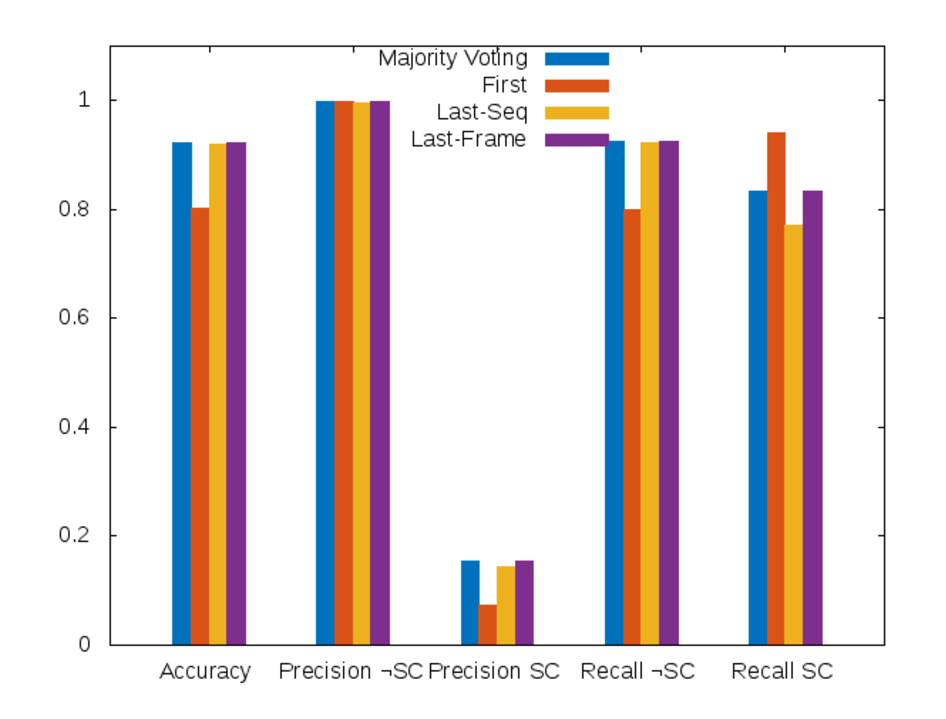
\includegraphics[scale=.7]{images/evalutation_net.eps}
	\caption{TODO: correct image?}
	\label{fig:evaluation_net}
\end{figure}
% TODO: die labels dieser Grafik sind nicht gut. die ganzen SCs stehen irgendwie immer so, dass sie zu mehreren Balken gehoeren koennten. Das mit dem not-Strich davor finde ich auch nicht schoen.
As the graphic shows the results ... TODO

Because we have such a low precision for soft cuts, we also tried to increase the value by trying out the \textit{Gap Filler}.
Unfortunately, this had no impact at all.
The precision of soft cuts did not increase.
TODO

Up to now we used a sequence length of eleven.
We decided to keep such low, so that we do not miss a soft cut.
TODO: explain better
The average soft cut length in the actual video data is however 21.
So we decided to test our architecture with a sequence length of 21.
TODO


